\documentclass{beamer}

\usepackage[utf8x]{inputenc}
\usepackage[OT4]{fontenc}

\usetheme[bullet=circle,
          titleline=true,
          pageofpages=of,
          alternativetitlepage=true]{Torino}

\usepackage{ragged2e}
\usepackage{hyphenat}
\usepackage{hyperref}
\usepackage{booktabs}

\usepackage{pgf,tikz}
\usepackage{pgfplots}

\usetikzlibrary{arrows}
\usetikzlibrary{automata}
\usetikzlibrary{backgrounds}
\usetikzlibrary{decorations}

\usepackage{amsmath}
\usepackage{amsfonts}
\usepackage{amsthm}

\definecolor{MyGreen}{rgb}{0.40,0.80,0.20}

\title{A New Online Interactive Web Notebook Based on ExtJS}
\author{Mateusz Paprocki \texttt{<mattpap@gmail.com>}}
\institute[PWR]{Wrocław University of Technology}
\date{\today}

\newenvironment{jblock}[1]{
    \begin{block}{#1}\justifying\nohyphens
}{
    \end{block}
}

\setbeamercovered{transparent}

\begin{document}

\frame{\titlepage}

\begin{frame}
    \frametitle{Presentation plan}
    \framesubtitle{}

    \begin{itemize}
        \item Approach to interaction with ...
    \end{itemize}
\end{frame}

\begin{frame}
    \frametitle{Classical approaches to interactive UIs}
    \framesubtitle{Introduction}

    \begin{itemize}
        \item aa
    \end{itemize}
\end{frame}

\begin{frame}
    \frametitle{Classical approaches to interactive UIs}
    \framesubtitle{Example: Terminal based approach}

    \begin{center}
        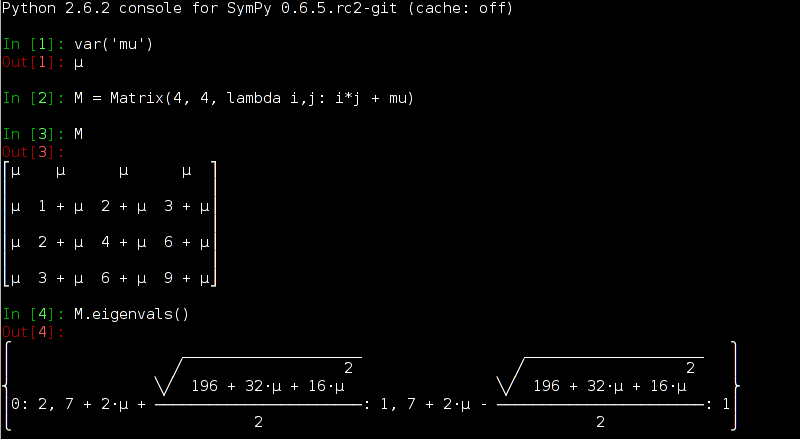
\includegraphics[scale=0.65]{images/sympy-unicode.png}
    \end{center}
\end{frame}

\begin{frame}
    \frametitle{Classical approaches to interactive UIs}
    \framesubtitle{Example: Windowing based approach}

    \begin{center}
        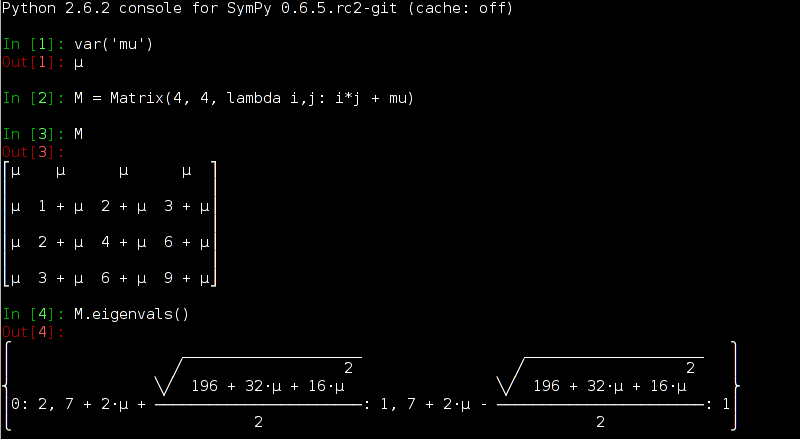
\includegraphics[scale=0.65]{images/sympy-unicode.png}
    \end{center}
\end{frame}

\begin{frame}
    \frametitle{Classical approaches to interactive UIs}
    \framesubtitle{Advantages and disadvantages}

    {\color{MyGreen} Pros}:
    \begin{itemize}
        \item mainly benefits for developers
            \begin{itemize}
                \item no problems with cross--browser compatibility
            \end{itemize}
    \end{itemize}
    \pause
    {\color{red} Cons}:
    \begin{itemize}
        \item user needs to install the program
    \end{itemize}
\end{frame}

\begin{frame}
    \frametitle{What is a web notebook?}
    \framesubtitle{}

    \begin{itemize}
        \item aa
    \end{itemize}
\end{frame}

\begin{frame}
    \frametitle{What is a web notebook?}
    \framesubtitle{}

    \begin{itemize}
        \item aa
    \end{itemize}
\end{frame}

\begin{frame}
    \frametitle{What is ExtJS?}
    \framesubtitle{}

    A \structure{web} development \structure{framework}:
    \pause
    \begin{itemize}
        \item allows for building rich internet applications
        \pause
        \item provides UI widgets in a browser window
        \pause
        \item cross--browser compatible
            \begin{itemize}
                \item Internet Explorer 6+
                \item FireFox 1.5+
                \item Safari 3+
                \item Chrome 3+
                \item Opera 9+
            \end{itemize}
        \pause
        \item dual licensed (GPL 3 and commercial)
        \pause
        \item available from \texttt{www.sencha.com}
    \end{itemize}
    \pause
    There are \structure{other} web development frameworks:
    \begin{itemize}
        \item Prototype, YUI, Dojo, MooTools, \structure{\ldots}
    \end{itemize}
\end{frame}

\begin{frame}
    \frametitle{What is Codenode?}
    \framesubtitle{}

    An \structure{interactive} online \structure{notebook}:
    \pause
    \begin{itemize}
        \item multiple--level architecture
            \begin{itemize}
                \item user web interface
                \pause
                \item frontend server
                \pause
                \item backend servers
            \end{itemize}
        \item support for \structure{Python} and \structure{Sage}
        \item use database for storing worksheets and other data
        \pause
        \item available from \texttt{www.codenode.org}
    \end{itemize}
    \pause
    There are \structure{other} web interactive notebooks:
    \begin{itemize}
        \item Sage Notebook (\texttt{www.sagenb.org}), \structure{\ldots}
    \end{itemize}
\end{frame}

\begin{frame}
    \frametitle{FEMhub Online Lab}
    \framesubtitle{}

    \begin{itemize}
        \item
    \end{itemize}
\end{frame}

\begin{frame}
    \frametitle{FEMhub Online Lab}
    \framesubtitle{}

    early stage of development

    component based design
     embed inside other web sites


    jsMath
\end{frame}

\begin{frame}
    \frametitle{Future plans}
    \framesubtitle{}

\end{frame}

\end{document}

